\newif\ifuseelsarticle
\IfFileExists{elsarticle.cls}{%
  \useelsarticletrue
  \documentclass[preprint,12pt]{elsarticle}
}{%
  \useelsarticlefalse
  \documentclass[12pt]{article}
}

\usepackage{amsmath}
\usepackage{amssymb}
\usepackage{booktabs}
\usepackage{float}
\usepackage{graphicx}
\usepackage[numbers,sort&compress]{natbib}
\usepackage{hyperref}
\usepackage{tikz}
\usepackage{caption}
\usepackage{subcaption}
\usetikzlibrary{positioning,arrows.meta}
\setlength{\emergencystretch}{2em}
\newcommand{\papertitle}{An open pseudo-3D Sleipner benchmark for temporal support inference}

\ifuseelsarticle
\journal{Journal of Applied Geophysics}
\biboptions{sort&compress}
\fi

\begin{document}

\ifuseelsarticle
\begin{frontmatter}

\title{\papertitle}

\author[inst1]{Ameer Alhashemi\corref{cor1}}
\ead{ameeralhashemi.ah@gmail.com}
\cortext[cor1]{Corresponding author}
\address[inst1]{University of Birmingham, Edgbaston, Birmingham B15 2TT, United Kingdom}

\begin{abstract}
Public field evaluation of time-lapse seismic change mapping remains limited, particularly for multi-inline assessment on open data. We construct an open pseudo-3D Sleipner benchmark from eleven neighboring inlines with two tracks: a p07 temporal branch (1994 to 2001, 2004, 2006) and a p10 direct branch (1994 to 2010). We introduce temporal support inference, constrained by public benchmark masks, that extends structured reconstruction with inline and temporal voting, probability blending, and monotone growth constraints. On a harder three-seed synthetic benchmark, plain machine learning is more stable than the hybrid model (Dice $0.544 \pm 0.008$ on the test split; $0.206 \pm 0.032$ out of distribution). On field data, temporal support inference increases p10 support-volume IoU from 0.562 for constrained plain machine learning and 0.685 for non-temporal structured reconstruction to 0.771, while retaining trace-support IoU at 0.907. On the p07 benchmark it increases support-volume IoU from 0.300 and 0.438 to 0.600, with trace-support IoU 0.910 and crossline continuity 0.986, while remaining far more selective than the constrained classical baseline. Reusing three saved seed artifacts without additional field training confirms mean support-volume IoU of $0.709 \pm 0.044$ on p10 and $0.587 \pm 0.025$ on p07. A secondary wave-temporal sweep shows that transfer passes a joint p10/p07 gate only at quantiles 0.74 and 0.75, and that low-memory adaptation can collapse occupancy. The benchmark therefore supports a reproducible evaluation protocol and a temporal support inference method.
\end{abstract}

\begin{keyword}
CO$_2$ storage monitoring \sep time-lapse seismic \sep Sleipner \sep pseudo-3D benchmark \sep temporal support inference \sep support mapping
\end{keyword}

\end{frontmatter}
\else
\title{\papertitle}
\author{Ameer Alhashemi}
\date{}
\begin{center}
{\LARGE\bfseries\parbox{0.88\textwidth}{\centering \papertitle\par}}
\vspace{1.6em}

{\Large Ameer Alhashemi\par}
\vspace{0.45em}

{University of Birmingham, Edgbaston, Birmingham B15 2TT, United Kingdom\par}
\vspace{0.35em}

{\normalsize\href{mailto:ameeralhashemi.ah@gmail.com}{ameeralhashemi.ah@gmail.com}\par}
\end{center}
\vspace{1.2em}

\begin{abstract}
Public field evaluation of time-lapse seismic change mapping remains limited, particularly for multi-inline assessment on open data. We construct an open pseudo-3D Sleipner benchmark from eleven neighboring inlines with two tracks: a p07 temporal branch (1994 to 2001, 2004, 2006) and a p10 direct branch (1994 to 2010). We introduce temporal support inference, constrained by public benchmark masks, that extends structured reconstruction with inline and temporal voting, probability blending, and monotone growth constraints. On a harder three-seed synthetic benchmark, plain machine learning is more stable than the hybrid model (Dice $0.544 \pm 0.008$ on the test split; $0.206 \pm 0.032$ out of distribution). On field data, temporal support inference increases p10 support-volume IoU from 0.562 for constrained plain machine learning and 0.685 for non-temporal structured reconstruction to 0.771, while retaining trace-support IoU at 0.907. On the p07 benchmark it increases support-volume IoU from 0.300 and 0.438 to 0.600, with trace-support IoU 0.910 and crossline continuity 0.986, while remaining far more selective than the constrained classical baseline. Reusing three saved seed artifacts without additional field training confirms mean support-volume IoU of $0.709 \pm 0.044$ on p10 and $0.587 \pm 0.025$ on p07. A secondary wave-temporal sweep shows that transfer passes a joint p10/p07 gate only at quantiles 0.74 and 0.75, and that low-memory adaptation can collapse occupancy. The benchmark therefore supports a reproducible evaluation protocol and a temporal support inference method.
\end{abstract}

\noindent\textbf{Keywords.} CO$_2$ storage monitoring; time-lapse seismic; Sleipner; pseudo-3D benchmark; temporal support inference; support mapping
\fi

\section{Introduction}

Time-lapse seismic data have played a central role in monitoring the Sleipner CO$_2$ storage site for nearly three decades \citep{furre2017sleipner}. The site is important not only because of its long injection history, but also because it has become one of the rare public field datasets where repeated seismic vintages, benchmark reservoir information, and interpreted plume products are available together \citep{equinor2020seismic,equinor2020benchmark}. This makes Sleipner a natural test case for methods that aim to move beyond qualitative difference maps toward more quantitative and reproducible change mapping.

At the same time, Sleipner is a difficult testbed. Repeated surveys are affected by non-repeatability, processing changes, tuning effects, and uncertainty in how seismic response relates to plume geometry \citep{rickett2001crossequalization,alali2020crossequalization,romero2023joint}. Recent work has shown that physics-based inversion and segmentation constraints can improve field interpretation, but the workflow remains demanding and the final field products still depend on strong structural information \citep{romero2023joint,fachtony2025sleipner}. Machine learning studies have also shown promise, including prior work on Sleipner interpretation and site-specific field transfer at other storage sites \citep{li2021sleipnernn,leong2024seisco2net}. However, there is still a gap between simplified synthetic demonstrations and open, field-facing, reproducible pseudo-3D evaluation on public CO$_2$ monitoring data.

This paper addresses that gap with three linked contributions. First, it constructs an open pseudo-3D Sleipner benchmark from eleven neighboring inlines while keeping the 2007 and 2010 processing families separate, thereby creating a transparent multi-inline public testbed for field evaluation. Second, it introduces benchmark-constrained temporal support inference, which converts section-wise probabilities into pseudo-3D support volumes using fixed inline, temporal, and support-volume constraints. Third, it retains a secondary operating-point protocol for wave-temporal deployment so that transfer claims can be stated conservatively rather than through one-off threshold choices.

The central research question is whether benchmark-constrained temporal support inference on public Sleipner data can improve field-facing support mapping beyond plain per-section machine learning and non-temporal structured reconstruction while remaining reproducible across reused seed artifacts. On the present benchmark, the clearest field result is that the temporal structured method gives the strongest support-volume mapping on both the direct p10 branch and the temporal p07 branch. The hybrid model remains secondary, and the wave-temporal gate study is retained only as a supporting deployment sensitivity analysis. The paper should therefore be read primarily as a benchmark-plus-method study rather than as a broad model comparison.

\section{Public data and benchmark construction}

\subsection{Public Sleipner data}

All field experiments use public data from the Sleipner 4D Seismic Dataset and the Sleipner 2019 Benchmark Model distributed through CO2DataShare \citep{equinor2020seismic,equinor2020benchmark}. The seismic dataset contains processed 4D seismic cubes from 1994 to 2010 and includes different processing families such as the 2007 and 2010 products. The benchmark model provides the reference simulation grid, velocity trends, reservoir horizons, and plume boundary products that allow public structural constraints to be aligned with the seismic data.

The benchmark construction uses inline exports from the processed seismic cubes. This choice is intentional and is aimed at establishing a transparent pseudo-3D monitoring benchmark from open data.

\subsection{Pseudo-3D benchmark design}

We construct two related but distinct field benchmarks from eleven contiguous inlines centered on inline 1840. The temporal benchmark uses the 2007 processing family and evaluates the 1994 baseline against the 2001, 2004, and 2006 monitor vintages. The direct benchmark uses matched 2010 processing and evaluates the 1994 baseline against the 2010 monitor. These two benchmarks are kept separate throughout the study because mixing processing families would confound temporal interpretation.

For every exported inline pair, we store a normalized baseline section, a normalized monitor section, a storage-interval mask derived from the public benchmark surfaces, a trace-support product based on the public 2010 plume outlines, and a 2D support-volume proxy aligned to the seismic section. The result is a pseudo-3D volume with dimensions inline, vintage, sample, and trace. This arrangement allows crossline continuity to be evaluated explicitly rather than inferred from a single section.

\begin{figure}[H]
\centering
\resizebox{0.97\textwidth}{!}{%
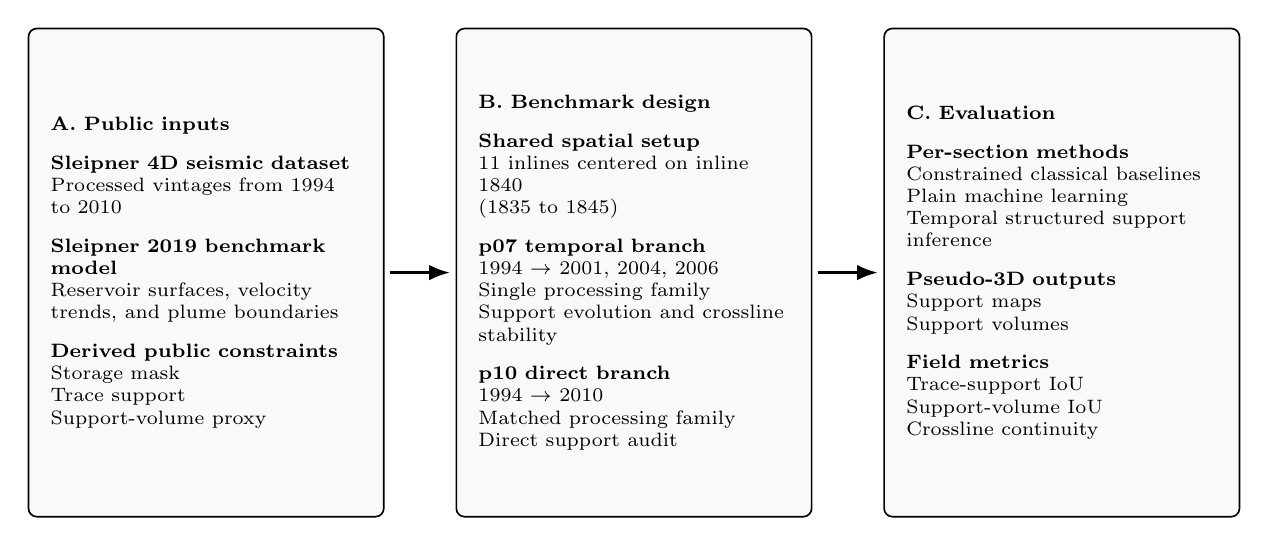
\begin{tikzpicture}[
  font=\scriptsize,
  box/.style={
    draw,
    rounded corners=3pt,
    line width=0.6pt,
    fill=gray!5,
    align=left,
    text width=3.95cm,
    inner sep=8pt,
    minimum height=6.2cm
  },
  flow/.style={-Latex, line width=1.0pt}
]
\node[box] (inputs) {
\textbf{A. Public inputs}\par\medskip
\textbf{Sleipner 4D seismic dataset}\par
Processed vintages from 1994 to 2010\par\medskip
\textbf{Sleipner 2019 benchmark model}\par
Reservoir surfaces, velocity trends, and plume boundaries\par\medskip
\textbf{Derived public constraints}\par
Storage mask\par
Trace support\par
Support-volume proxy
};
\node[box, right=0.9cm of inputs] (design) {
\textbf{B. Benchmark design}\par\medskip
\textbf{Shared spatial setup}\par
11 inlines centered on inline 1840\\
(1835 to 1845)\par\medskip
\textbf{p07 temporal branch}\par
1994 $\rightarrow$ 2001, 2004, 2006\par
Single processing family\par
Support evolution and crossline stability\par\medskip
\textbf{p10 direct branch}\par
1994 $\rightarrow$ 2010\par
Matched processing family\par
Direct support audit
};
\node[box, right=0.9cm of design] (evaluation) {
\textbf{C. Evaluation}\par\medskip
\textbf{Per-section methods}\par
Constrained classical baselines\par
Plain machine learning\par
Temporal structured support inference\par\medskip
\textbf{Pseudo-3D outputs}\par
Support maps\par
Support volumes\par\medskip
\textbf{Field metrics}\par
Trace-support IoU\par
Support-volume IoU\par
Crossline continuity
};
\draw[flow, shorten <=2pt, shorten >=2pt] (inputs.east) -- (design.west);
\draw[flow, shorten <=2pt, shorten >=2pt] (design.east) -- (evaluation.west);
\end{tikzpicture}
}
\caption{Public pseudo-3D benchmark design and evaluation protocol. Panel A summarizes the public seismic and benchmark products used to derive structural constraints. Panel B defines the two benchmark tracks used in the study. Panel C shows how constrained classical baselines, plain machine learning, and temporal structured support inference are evaluated through pseudo-3D support outputs and field metrics.}
\label{fig:benchmarkdesign}
\end{figure}

\subsection{Harder synthetic benchmark}

The synthetic benchmark used here serves as a stress test for model stability. Compared with the earlier toy benchmark, the current synthetic benchmark introduces stronger mismatch behavior, negative controls, and out-of-zone changes. In particular, we evaluate clean examples, harder out-of-distribution examples, and negative-control scenarios including no-change, mismatch-only, and out-of-zone cases. These synthetic experiments make it possible to evaluate model stability and false alarms across multiple random seeds in a way that cannot be achieved on the fixed field data alone.

\section{Methods}

\subsection{Method overview}

The study design is summarized in Fig.~\ref{fig:benchmarkdesign}. Public seismic and benchmark products are first converted into a pseudo-3D benchmark, after which constrained classical baselines and machine learning models are evaluated under the same structural constraints. The field-facing output is a support-mapping product defined on a shared pseudo-3D benchmark.

\subsection{Per-section methods}

We compare three method families at the per-section stage. The deterministic classical family includes difference, normalized root-mean-square difference, impedance difference, cross-equalized difference, local warp difference, and matched warp-shift difference. Each classical score is thresholded with the threshold that maximizes validation-set intersection-over-union on the harder synthetic benchmark, after which the thresholded field output is passed through the same reservoir-mask and connected-component cleanup used for constrained outputs. For each field pair, \emph{best classical constrained} denotes the thresholded classical candidate with the highest support-volume intersection-over-union against the benchmark support volume; if a support-volume proxy is unavailable, trace-support intersection-over-union is used instead. This rule is fixed in code and is not tuned separately for p07 and p10.

The two learned per-section models are plain machine learning and a hybrid model with additional engineered inputs. The synthetic sweep identifies the plain learner as the stronger base model, so the main field method is built on the plain probabilities. The hybrid model is retained as a comparator and negative result.

\subsection{Benchmark-constrained structured reconstruction}

The non-temporal structured baseline reconstructs support independently within each vintage after the per-section constrained plain-machine-learning output is available. For each vintage, the eleven inlines are grouped into a pseudo-3D volume and an active trace-support mask is obtained by majority voting across neighboring inlines with window size 3 and vote fraction 0.34. For each active trace, the vertical support column is reconstructed from the plain probabilities after Gaussian smoothing with $\sigma=1.25$. The local column profile is blended with the mean probability of adjacent inlines using a fixed 70:30 mixture. The reconstructed interval is then taken as the largest connected 1D component above a relative threshold of 0.45 times the local peak, with minimum peak probability 0.50 and a vertical dilation margin of 2 samples. The reported structured baseline uses no final morphological opening or closing and no component truncation.

\subsection{Benchmark-constrained temporal support inference}

The proposed method extends structured reconstruction into a pseudo-3D temporal inference problem. Starting from the structured plain result as a seed, the plain-model probabilities are assembled into a 4D array over vintage, inline, sample, and trace. Trace support is expanded by inline-majority voting (window size 3, vote fraction 0.34) and temporal-majority voting across vintages (window size 3, vote fraction 0.34). The active trace-support mask is then accumulated forward in time to enforce monotone support growth.

Within each active trace, the probability profile for the current vintage is blended with the mean probability of neighboring inlines (weight 0.20), the mean probability of neighboring vintages (weight 0.35), and the benchmark support-volume prior (weight 0.08). The resulting column is reconstructed with Gaussian smoothing $\sigma=1.0$, relative threshold 0.42, minimum peak probability 0.45, and vertical dilation margin 2. Support that emerges relative to the previous vintage is retained only if it overlaps the previous support column after one-sample dilation or if its local probability exceeds 0.52. The final 4D hypervolume is clipped to the reservoir mask and reported without additional morphological closing or component pruning in the main configuration.

We also tested a layer-aware extension that split the storage interval into benchmark-informed bands and enforced stronger vertical rules. That extension did not improve the field benchmark and is therefore retained only as a negative control.

\subsection{Evaluation metrics}

Synthetic experiments are reported using Dice, intersection-over-union, false-positive rate, and expected calibration error. Because the synthetic benchmark includes repeated training, the machine learning models are summarized with three-seed mean and standard deviation. Deterministic classical baselines are reported once because they do not depend on training seeds.

Field experiments are evaluated with metrics that are more appropriate for pseudo-3D monitoring. These include trace-support intersection-over-union with the public 2010 support proxy, support-volume intersection-over-union, crossline continuity, predicted trace fraction, and predicted fraction outside the support volume. The direct 2010 benchmark is treated as the main truth test because it compares seismic data and support proxy within the same processing family. The p07 temporal benchmark is used to test whether the inferred support remains selective, temporally consistent, and crossline coherent across the earlier monitor vintages.

\section{Experimental design}

The experiments are organized around four questions. The first asks whether the per-section models are stable on the harder synthetic benchmark. The second asks whether benchmark-constrained structured reconstruction improves pseudo-3D field mapping on the direct eleven-inline benchmark. The third asks whether the proposed temporal support inference stage improves the temporal eleven-inline benchmark relative to both plain machine learning and the non-temporal structured baseline. The fourth asks whether a fixed-artifact quantile protocol can still identify conservative cross-benchmark operating points for the separate wave-temporal comparator while avoiding unstable adaptation behavior.

For synthetic evaluation, we retrain the plain and hybrid models with seeds 11, 12, and 13. For field evaluation, all methods operate on the same exported pseudo-3D benchmarks and the same public support constraints. To test whether the main field claim is tied to a single trained artifact, the p07 and p10 benchmarks are also re-evaluated using the saved seed-11, seed-12, and seed-13 artifact roots from the harder synthetic sweep, with no additional field training. This keeps the comparison focused on the mapping method rather than on manual changes to the data pipeline.

\section{Results}

\subsection{Three-seed synthetic evaluation}

The three-seed sweep shows that plain machine learning is currently the more stable and stronger learner on the harder synthetic benchmark. On the test split, plain machine learning reaches a mean Dice of $0.544 \pm 0.008$, compared with $0.494 \pm 0.064$ for the hybrid model. On the out-of-distribution split, plain machine learning reaches $0.206 \pm 0.032$, compared with $0.166 \pm 0.024$ for the hybrid model. The strongest deterministic classical baseline on the out-of-distribution split remains the simple difference map at 0.108 Dice. These results are summarized in Table~\ref{tab:synthetic}.

\begin{table}[t]
\centering
\small
\caption{Synthetic benchmark results. Classical results are deterministic. Machine learning results are reported as mean $\pm$ standard deviation across three seeds.}
\label{tab:synthetic}
\resizebox{\textwidth}{!}{%
\begin{tabular}{llcccc}
\toprule
Split & Method & Dice & IoU & False-positive rate & ECE \\
\midrule
Test & Difference & 0.099 & 0.052 & 0.140 & 0.143 \\
Test & Plain ML & 0.544 $\pm$ 0.008 & 0.374 $\pm$ 0.008 & 0.011 $\pm$ 0.003 & 0.048 $\pm$ 0.016 \\
Test & Hybrid ML & 0.494 $\pm$ 0.064 & 0.331 $\pm$ 0.059 & 0.012 $\pm$ 0.003 & 0.043 $\pm$ 0.013 \\
\midrule
OOD & Difference & 0.108 & 0.057 & 0.065 & 0.073 \\
OOD & Plain ML & 0.206 $\pm$ 0.032 & 0.115 $\pm$ 0.020 & 0.004 $\pm$ 0.001 & 0.034 $\pm$ 0.019 \\
OOD & Hybrid ML & 0.166 $\pm$ 0.024 & 0.091 $\pm$ 0.014 & 0.006 $\pm$ 0.002 & 0.030 $\pm$ 0.013 \\
\bottomrule
\end{tabular}
}
\end{table}

The synthetic sweep clarifies the model comparison and identifies plain machine learning as the base learner that should be carried into the field evaluation.

\subsection{Direct eleven-inline benchmark}

The direct p10 benchmark is the clearest field result in the paper. Table~\ref{tab:direct} shows that non-temporal structured reconstruction improves support-volume intersection-over-union from 0.562 for constrained plain machine learning to 0.685, and the temporal support inference stage improves it further to 0.771 while keeping trace-support overlap essentially unchanged at 0.907. The predicted trace fraction remains nearly identical across the two learned support-mapping variants (0.352 for both structured methods), which means the p10 gain is not produced by indiscriminate support growth. The constrained classical baseline is much less selective, occupying 99.0\% of traces and placing 62.3\% of its predicted support outside the benchmark support volume.

\begin{table}[t]
\centering
\small
\caption{Direct eleven-inline p10 benchmark. The temporal support inference method yields the strongest support-volume result while preserving trace-support overlap and lateral support alignment.}
\label{tab:direct}
\resizebox{\textwidth}{!}{%
\begin{tabular}{lccccc}
\toprule
Method & Predicted trace fraction & Trace-support IoU & Support-volume IoU & Crossline continuity & Fraction outside support \\
\midrule
Best classical constrained & 0.990 & 0.322 & 0.363 & 0.987 & 0.623 \\
Plain ML constrained & 0.351 & 0.910 & 0.562 & 0.973 & 0.018 \\
Plain ML structured constrained & 0.352 & 0.907 & 0.685 & 0.977 & 0.025 \\
Plain ML temporal structured constrained & 0.352 & 0.907 & 0.771 & 0.978 & 0.028 \\
\bottomrule
\end{tabular}
}
\end{table}

Figure~\ref{fig:directpanel} illustrates this result on inline 1840. The temporal method retains the compact geometry of the structured baseline while recovering more of the benchmark support extent. The layer-aware extension remained weaker and is discussed later only as a negative control.

\begin{figure}[H]
\centering
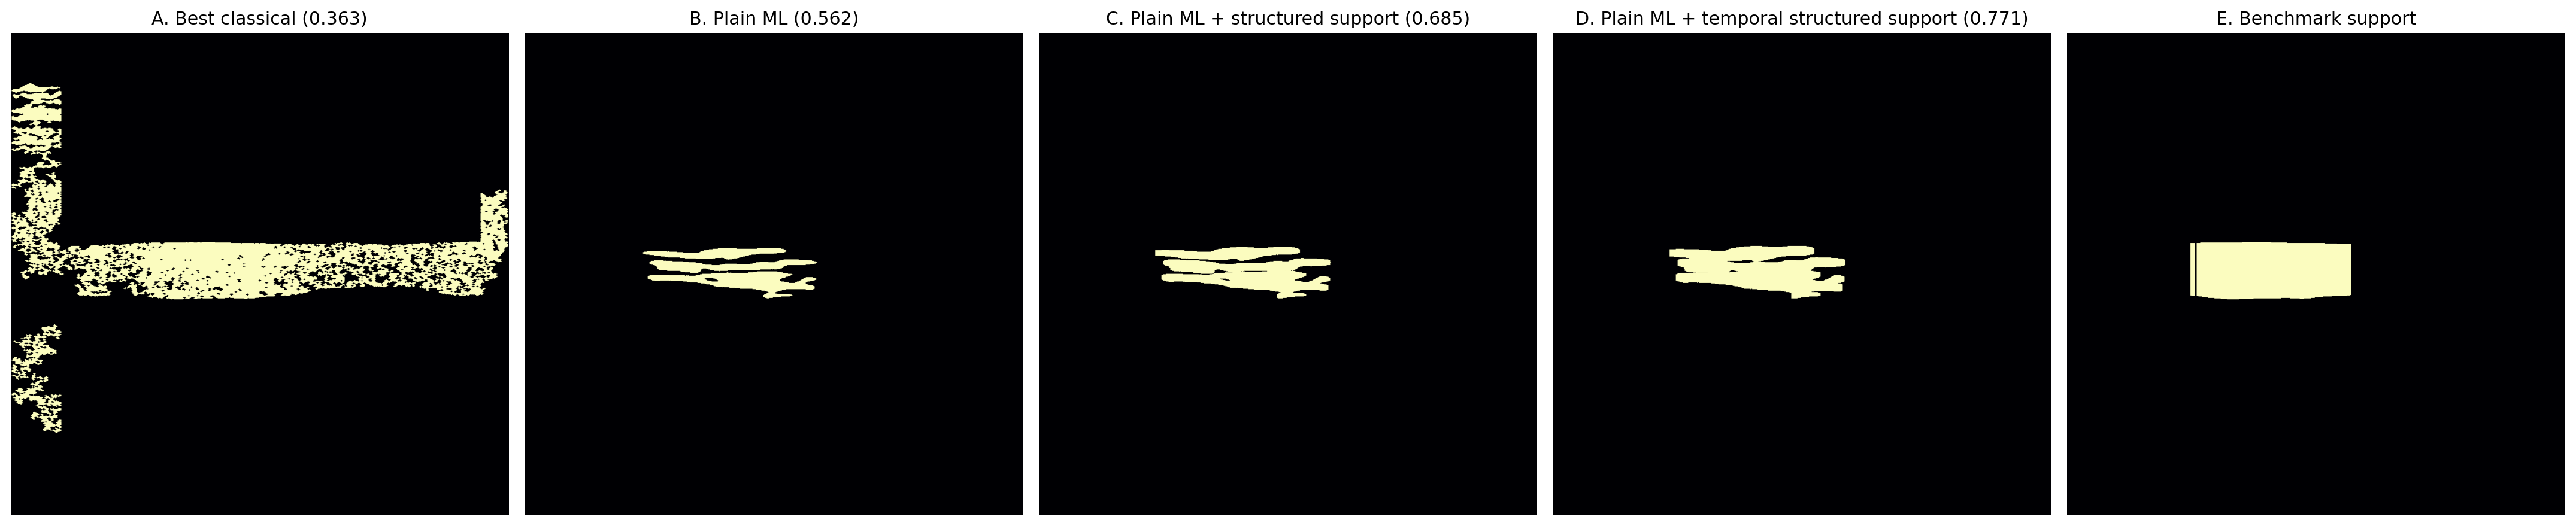
\includegraphics[width=\textwidth]{figures/paper_direct_2010_panel.png}
\caption{Direct p10 benchmark on inline 1840. From left to right the panels show the best constrained classical baseline, constrained plain machine learning, constrained plain machine learning with non-temporal structured reconstruction, constrained plain machine learning with temporal support inference, and the benchmark support. The temporal support inference method provides the strongest support-volume agreement on the direct benchmark.}
\label{fig:directpanel}
\end{figure}

\subsection{Temporal eleven-inline benchmark}

The p07 temporal benchmark is where temporal coupling matters most. Across the full eleven-inline volume, the constrained classical baseline attains support-volume intersection-over-union of 0.477 by predicting support on almost the entire permitted trace set: its predicted trace fraction is 0.995 and 48.8\% of the predicted support lies outside the public support proxy. Plain machine learning is much more selective but under-fills the support volume. Non-temporal structured reconstruction improves this balance, and the temporal support inference stage improves it further, reaching support-volume intersection-over-union of 0.600 with trace-support overlap of 0.910 and crossline continuity of 0.986 while keeping the predicted trace fraction to 0.359. Table~\ref{tab:temporal} summarizes these overall results, and Fig.~\ref{fig:fieldsummary} later shows the same p07 trade-off in a compact selectivity-performance view.

\begin{table}[t]
\centering
\small
\caption{Overall results on the eleven-inline p07 temporal benchmark. The temporal support inference method improves support-volume and trace-support agreement while remaining much more selective than the constrained classical baseline.}
\label{tab:temporal}
\resizebox{\textwidth}{!}{%
\begin{tabular}{lccccc}
\toprule
Method & Predicted trace fraction & Trace-support IoU & Support-volume IoU & Crossline continuity & Fraction outside support \\
\midrule
Best classical constrained & 0.995 & 0.385 & 0.477 & 0.998 & 0.488 \\
Plain ML constrained & 0.339 & 0.873 & 0.300 & 0.967 & 0.001 \\
Plain ML structured constrained & 0.342 & 0.879 & 0.438 & 0.982 & 0.002 \\
Plain ML temporal structured constrained & 0.359 & 0.910 & 0.600 & 0.986 & 0.005 \\
\bottomrule
\end{tabular}
}
\end{table}

The temporal slices in Fig.~\ref{fig:p07panel} show that the temporal method preserves a compact and coherent support geometry across the 2001, 2004, and 2006 monitors while following the public 2010 support envelope. The inferred support remains benchmark-constrained and is interpreted here as a support-mapping product rather than as a saturation estimate.

\begin{figure}[H]
\centering
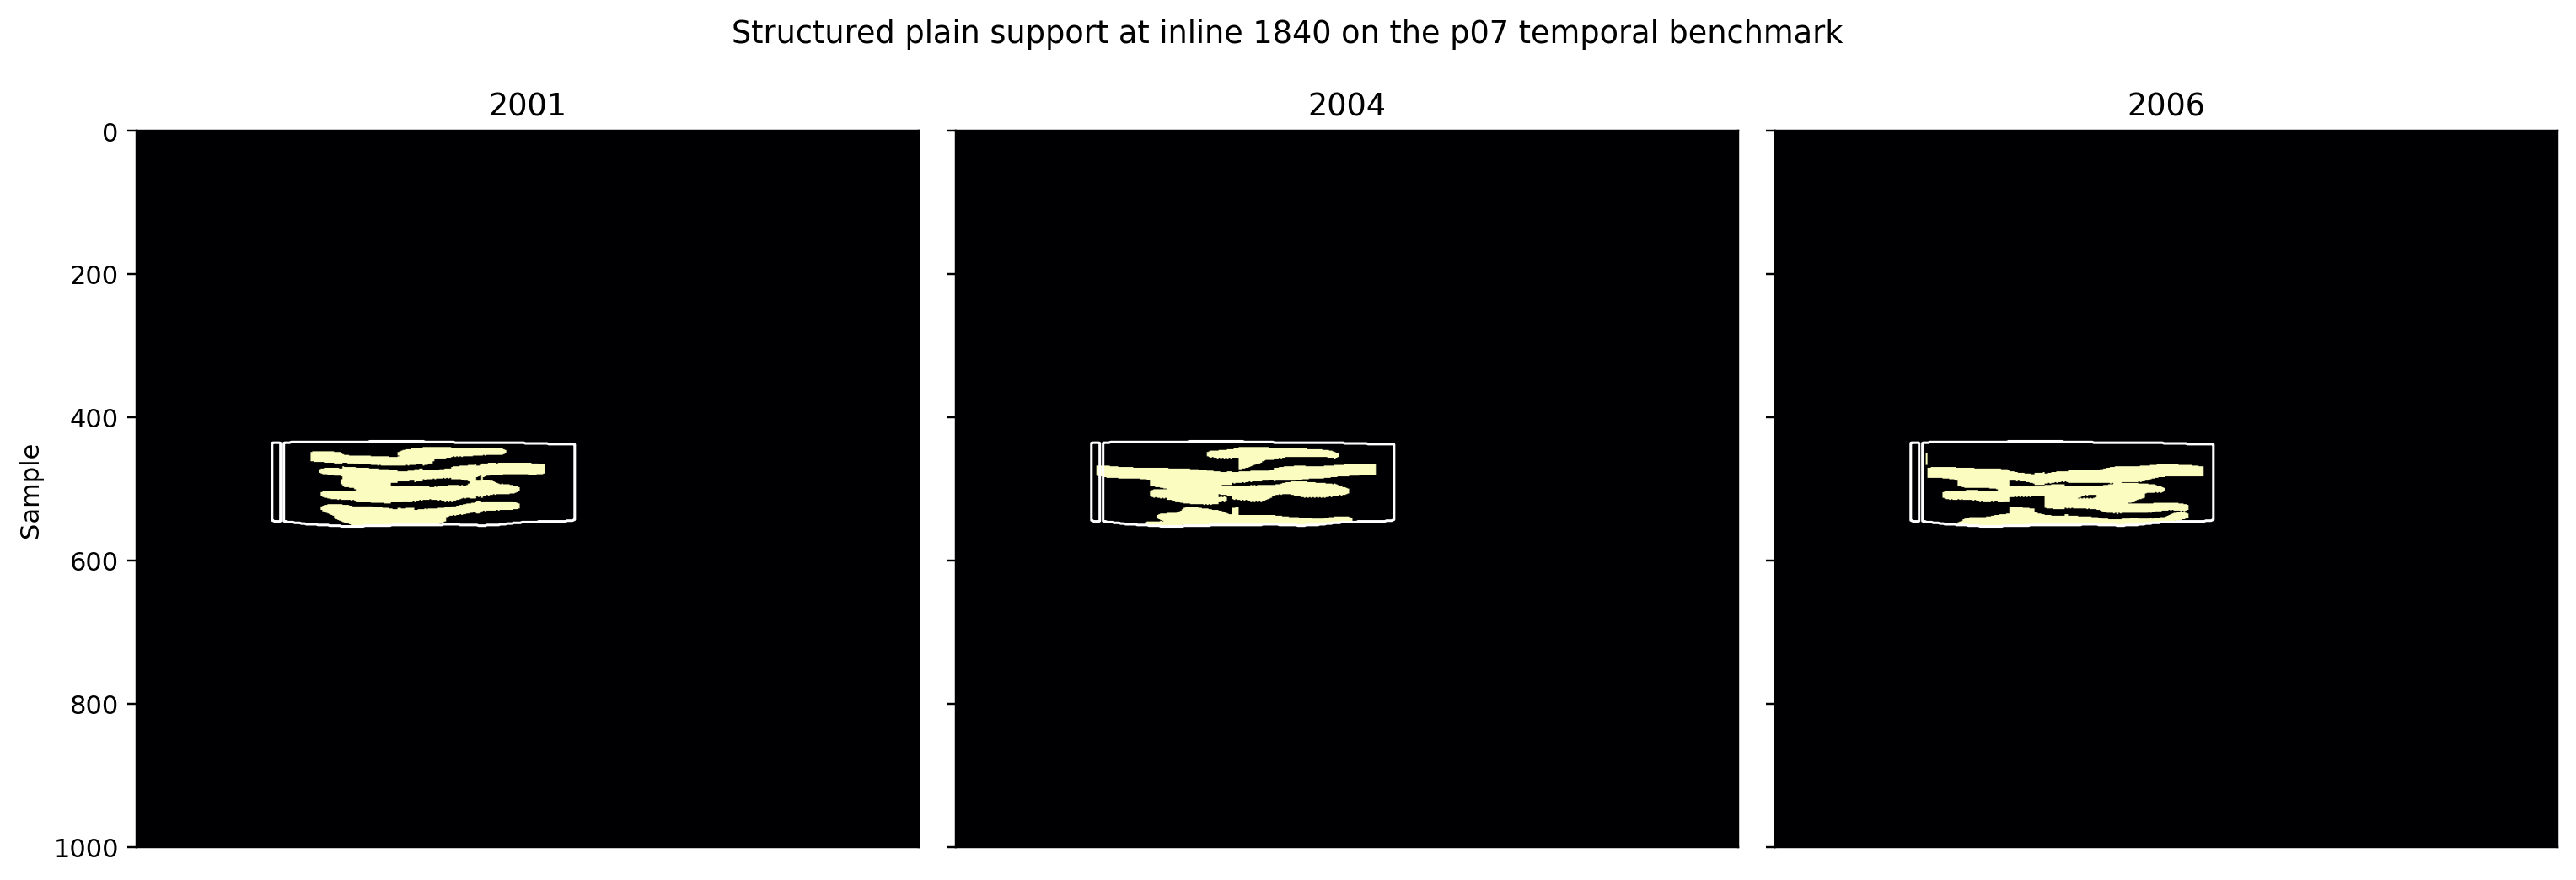
\includegraphics[width=0.95\textwidth]{figures/p07_temporal_panel.png}
\caption{Temporal structured support maps on inline 1840 for the p07 temporal benchmark. White contours show the public 2010 support proxy. The inferred support remains compact across vintages while expanding in a benchmark-constrained manner.}
\label{fig:p07panel}
\end{figure}

\subsection{Three-seed field stability of the main field baselines}

To test whether the main field conclusion depends on a single trained artifact, we re-evaluated the direct p10 and temporal p07 benchmarks with the saved seed-11, seed-12, and seed-13 artifacts from the harder synthetic sweep and no additional field training. Table~\ref{tab:fieldstability} shows that the temporal method remains the strongest support-volume variant on both branches. On p10, mean support-volume IoU rises from $0.526 \pm 0.048$ for plain machine learning and $0.637 \pm 0.037$ for the non-temporal structured baseline to $0.709 \pm 0.044$ for the temporal method. On p07, the temporal method increases mean support-volume IoU to $0.587 \pm 0.025$, above both non-temporal structured reconstruction ($0.440 \pm 0.052$) and the constrained classical baseline (0.477). The mean p07 trace-support IoU also rises to $0.925 \pm 0.010$.

This stability check sharpens the interpretation of the field results. The direct p10 branch supports a robust support-volume claim for temporal support inference. The p07 branch shows the same method advantage, although the mean crossline continuity of the temporal method ($0.959 \pm 0.020$) is slightly lower than that of the non-temporal structured baseline ($0.969 \pm 0.011$). The trade-off is therefore not hidden: the temporal method gains support-volume agreement and trace-support overlap while maintaining high, though not maximal, crossline continuity.

\begin{table}[t]
\centering
\small
\caption{Three-seed field stability check using the saved seed-11, seed-12, and seed-13 artifacts and no additional field training. Values are mean $\pm$ standard deviation across the three seed artifacts.}
\label{tab:fieldstability}
\resizebox{\textwidth}{!}{%
\begin{tabular}{llcccc}
\toprule
Benchmark & Method & SV IoU & Trace-support IoU & Crossline continuity & Fraction outside support \\
\midrule
p07 & Best classical constrained & 0.477 $\pm$ 0.000 & 0.385 $\pm$ 0.000 & 0.998 $\pm$ 0.000 & 0.488 $\pm$ 0.000 \\
p07 & Plain ML constrained & 0.304 $\pm$ 0.061 & 0.886 $\pm$ 0.012 & 0.956 $\pm$ 0.009 & 0.003 $\pm$ 0.002 \\
p07 & Plain ML structured constrained & 0.440 $\pm$ 0.052 & 0.890 $\pm$ 0.012 & 0.969 $\pm$ 0.011 & 0.007 $\pm$ 0.006 \\
p07 & Plain ML temporal structured constrained & 0.587 $\pm$ 0.025 & 0.925 $\pm$ 0.010 & 0.959 $\pm$ 0.020 & 0.013 $\pm$ 0.009 \\
\midrule
p10 & Best classical constrained & 0.363 $\pm$ 0.000 & 0.322 $\pm$ 0.000 & 0.987 $\pm$ 0.000 & 0.623 $\pm$ 0.000 \\
p10 & Plain ML constrained & 0.526 $\pm$ 0.048 & 0.794 $\pm$ 0.158 & 0.863 $\pm$ 0.142 & 0.072 $\pm$ 0.077 \\
p10 & Plain ML structured constrained & 0.637 $\pm$ 0.037 & 0.770 $\pm$ 0.188 & 0.924 $\pm$ 0.065 & 0.096 $\pm$ 0.100 \\
p10 & Plain ML temporal structured constrained & 0.709 $\pm$ 0.044 & 0.770 $\pm$ 0.188 & 0.926 $\pm$ 0.064 & 0.103 $\pm$ 0.104 \\
\bottomrule
\end{tabular}
}
\end{table}

Figure~\ref{fig:fieldsummary} summarizes the same stability result in two compact views. Panel A confirms that the temporal method is the strongest support-volume method across both benchmark branches in the reused three-seed evaluation. Panel B shows that the p07 gain is not obtained by indiscriminate over-occupancy: the temporal method moves to higher support-volume agreement while remaining far more selective than the constrained classical baseline.

\begin{figure}[t]
\centering
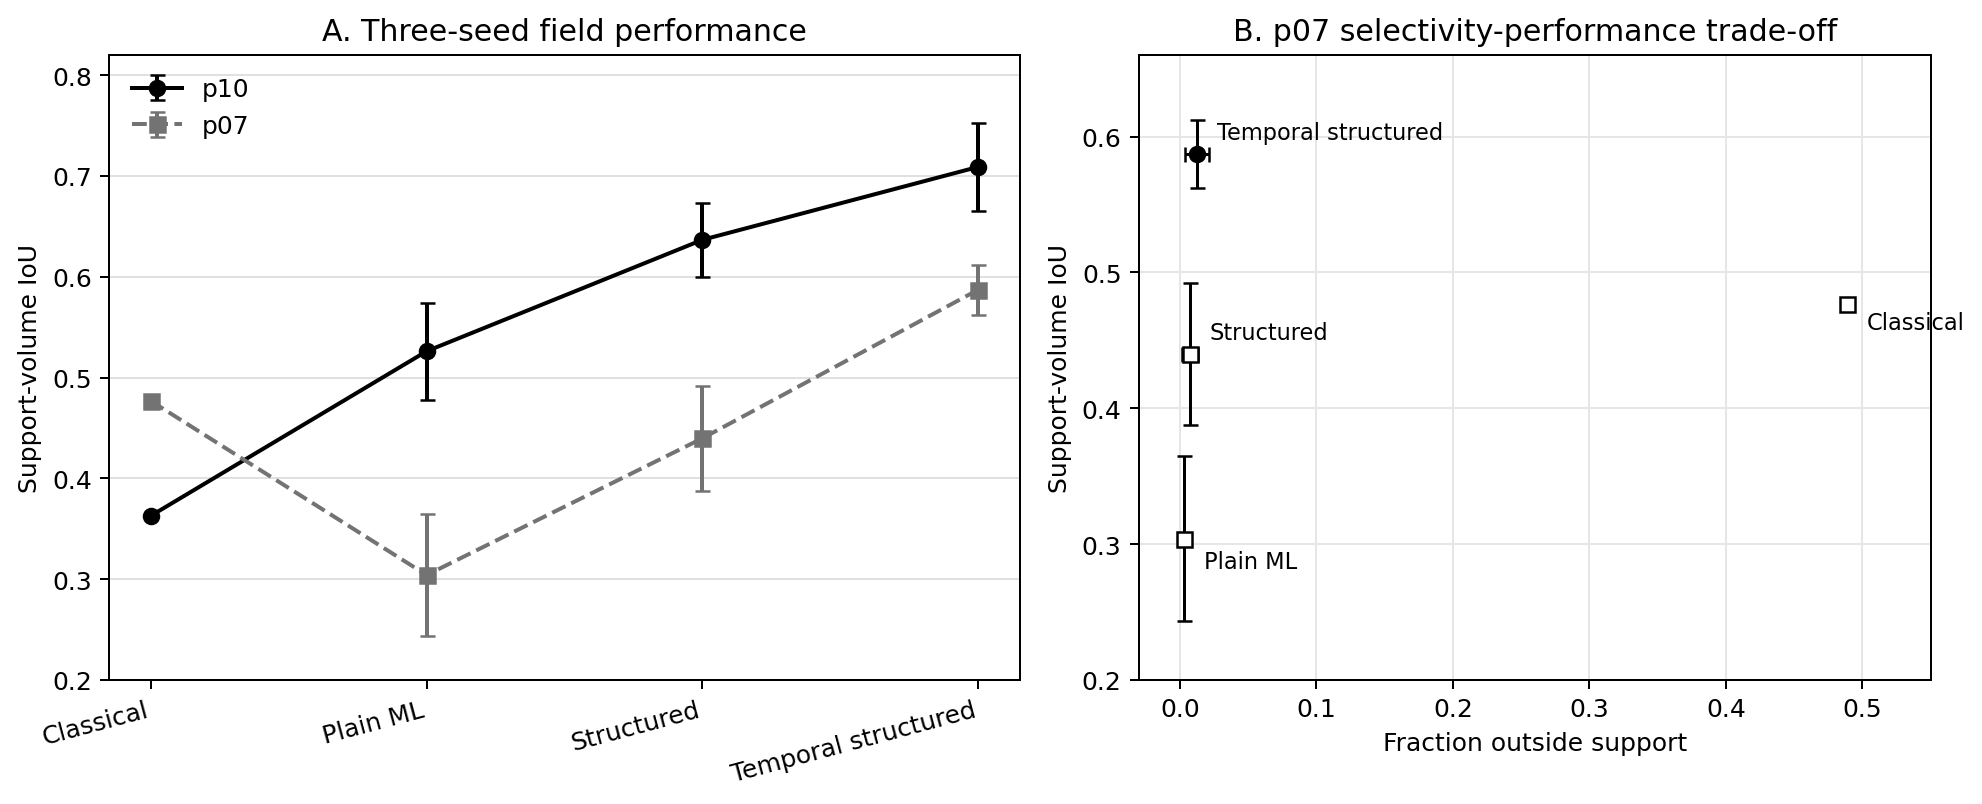
\includegraphics[width=\textwidth]{figures/paper_field_summary_panel.png}
\caption{Quantitative summary of the three-seed field stability evaluation. Panel A shows mean $\pm$ standard deviation of support-volume intersection-over-union across the p07 and p10 benchmarks for the main field baselines. Panel B shows the p07 selectivity-performance trade-off between support-volume agreement and the fraction of predicted support outside the public support proxy. The temporal support inference method improves support-volume agreement while remaining far more selective than the constrained classical baseline.}
\label{fig:fieldsummary}
\end{figure}

\subsection{Secondary wave-temporal deployment sensitivity analysis}

An additional field check was retained only to define a conservative deployment protocol for the separate wave-temporal comparator. In low-memory mode with field adaptation enabled, support occupancy collapsed on both branches: at quantile 0.82, p10 support-volume intersection-over-union fell from 0.526 to 0.000 and p07 fell from 0.159 to 0.000, while the predicted fraction outside support rose to 1.000 in both cases. We therefore fixed the training artifacts and disabled field adaptation for the comparator sweep.

Under that fixed-artifact protocol, a three-seed quantile sweep on $q \in [0.74, 0.80]$ kept p10 support-volume intersection-over-union above constrained classical at every tested quantile (0.570 versus 0.345), whereas p07 met or exceeded constrained classical only at quantiles 0.74 and 0.75, with margins of +0.024 and +0.013. Table~\ref{tab:gate} summarizes the resulting gate decision.

\begin{table}[t]
\centering
\small
\caption{Cross-benchmark gate for wave-temporal deployment with fixed training artifacts and no field adaptation (three-seed means). Gate condition: p10 support-volume IoU $>$ constrained classical and p07 support-volume IoU $\geq$ constrained classical.}
\label{tab:gate}
\resizebox{\textwidth}{!}{%
\begin{tabular}{ccccccc}
\toprule
Quantile & p10 wave SV IoU & p10 classical SV IoU & p07 wave SV IoU & p07 classical SV IoU & p10 margin & p07 margin \\
\midrule
0.74 & 0.570 & 0.345 & 0.431 & 0.407 & +0.225 & +0.024 \\
0.75 & 0.570 & 0.345 & 0.420 & 0.407 & +0.225 & +0.013 \\
0.76 & 0.570 & 0.345 & 0.406 & 0.407 & +0.225 & -0.001 \\
0.77 & 0.570 & 0.345 & 0.394 & 0.407 & +0.225 & -0.012 \\
0.78 & 0.570 & 0.345 & 0.380 & 0.407 & +0.225 & -0.027 \\
0.79 & 0.570 & 0.345 & 0.364 & 0.407 & +0.225 & -0.042 \\
0.80 & 0.570 & 0.345 & 0.346 & 0.407 & +0.225 & -0.061 \\
\bottomrule
\end{tabular}
}
\end{table}

The pass region is therefore narrow but reproducible. Quantile 0.74 is selected as the primary operating point, with 0.75 retained as a sensitivity check. This result is included only as a secondary deployment sensitivity analysis for the wave-temporal comparator.

\subsection{Negative results and false alarms}

Three negative results are important to retain. First, the hybrid model does not outperform plain machine learning on the harder synthetic benchmark and remains weaker on the direct field benchmark. Second, the layer-aware extension does not improve the field result and reduces both trace-support overlap and crossline continuity. Third, low-memory field adaptation can collapse wave-temporal support occupancy in this setting, which makes adaptation safety checks necessary before deployment. These outcomes help define the scope of the contribution supported by the present benchmark.

The negative-control synthetic scenarios also reinforce this point. On mismatch-only and out-of-zone examples, plain machine learning keeps the false-positive rate low while retaining higher Dice than the hybrid model for out-of-zone changes. These scenarios do not replace field validation, but they show that the benchmark can reject weak hypotheses as well as confirm positive results.

\section{Discussion}

The main result is that the open benchmark supports a method claim, not only a benchmarking claim. Benchmark-constrained temporal support inference converts stable section-level probabilities into pseudo-3D support volumes that outperform both plain machine learning and non-temporal structured reconstruction on the direct and temporal branches. On p10 the gain is primarily volumetric: support-volume agreement rises strongly while trace-support overlap remains essentially unchanged. On p07 the gain comes from coupling inline and vintage context. The temporal method increases support-volume and trace-support agreement while keeping the predicted trace fraction far below the near-saturated classical occupancy.

The benchmark contribution remains important because the method depends on it. Public inline exports, public structural constraints, and pseudo-3D metrics make it possible to test whether a support-mapping method is merely producing large occupied regions or is actually delivering coherent and selective monitoring products. The constrained classical baseline illustrates this point clearly on p07: its raw support-volume score is respectable only because it occupies nearly the entire permitted trace set and still places a large fraction of support outside the benchmark proxy. Without the pseudo-3D benchmark, this failure mode would be harder to diagnose.

The secondary wave-temporal gate study should be interpreted more narrowly. It shows that a separate comparator can require explicit operating-point control and adaptation sanity checks before deployment. That study does not carry the novelty of the paper on its own, but it does reinforce the broader argument that field-facing CO$_2$ monitoring claims should be benchmarked under explicit constraints and transfer rules.

Several limitations remain. The field results are benchmark-constrained and should be interpreted as support mapping. The pseudo-3D benchmark is assembled from multiple inlines rather than from the full 3D field cube. The support-volume proxy is benchmark-derived and evaluates support occupancy rather than direct saturation. The synthetic benchmark is more demanding than the earlier version, but it still does not represent full site-scale coupled flow and wave physics. Even with these limitations, the study provides an open-data testbed for comparing field-facing CO$_2$ monitoring methods under shared constraints and shared metrics.

These findings also have a practical implication for CCS monitoring. Open field evaluation benefits from metrics that reward spatial selectivity, temporal consistency, and crossline coherence in addition to section-wise agreement. In that setting, benchmark-constrained temporal support inference converts stable section-level probabilities into pseudo-3D support volumes that are easier to audit against public benchmark products and more interpretable as monitoring outputs.

\section{Conclusions}

This paper introduced an open pseudo-3D Sleipner benchmark for time-lapse CO$_2$ monitoring and used it to test benchmark-constrained temporal support inference under separate temporal and direct evaluation settings. The benchmark was used to compare constrained classical baselines, plain machine learning, hybrid machine learning, non-temporal structured reconstruction, and the proposed temporal support inference stage.

The main findings are straightforward. Plain machine learning is more stable than the hybrid model on the harder three-seed synthetic benchmark. Benchmark-constrained temporal support inference gives the strongest support-volume result on the direct p10 pseudo-3D benchmark, increasing support-volume IoU to 0.771 in the main run and to $0.709 \pm 0.044$ across reused seed artifacts. On the p07 temporal benchmark, the same method raises support-volume IoU to 0.600 in the main run and to $0.587 \pm 0.025$ across reused seed artifacts, while retaining high trace-support overlap and crossline coherence. The layer-aware extension does not improve the benchmark. A secondary fixed-artifact gate check shows that the separate wave-temporal comparator satisfies both constrained-classical conditions only at quantiles 0.74 and 0.75, and that low-memory adaptation is otherwise unstable. The strongest conclusion supported by the present results is therefore that the open benchmark enables a reproducible field-facing method claim: temporal support inference materially improves pseudo-3D support mapping on both Sleipner benchmark branches.

The most valuable next step is broader evaluation against additional practical baselines and, if possible, an extension from pseudo-3D support mapping toward more directly quantitative field products.

\section*{Data and code availability}

The field data used in this study are publicly available through the Sleipner 4D Seismic Dataset and the Sleipner 2019 Benchmark Model on CO2DataShare \citep{equinor2020seismic,equinor2020benchmark}. The code used to construct the benchmark, run the reported experiments, and generate the manuscript figures and tables is available at \href{https://github.com/TallowCatch/Propagation}{github.com/TallowCatch/Propagation}. The frozen submission snapshot is identified in that repository as tag \texttt{jag-submission-2026-04-03}; \texttt{CITATION.cff} and \texttt{.zenodo.json} provide release metadata for archival citation. The accompanying reproducibility materials include the synthetic seed sweep, the three-seed field-stability tables, and the cross-benchmark operating-point and adaptation-check tables used in the manuscript.

\section*{CRediT authorship contribution statement}

Ameer Alhashemi: Conceptualization, Data curation, Formal analysis, Investigation, Methodology, Software, Validation, Visualization, Writing -- original draft, Writing -- review and editing.

\section*{Funding}

This research did not receive any specific grant from funding agencies in the public, commercial, or not-for-profit sectors.

\section*{Declaration of competing interest}

The author declares that there are no known competing financial interests or personal relationships that could have appeared to influence the work reported in this paper.

\section*{Declaration of generative AI and AI-assisted technologies in the writing process}

Generative AI tools were used only to assist with language editing and manuscript organization. All scientific claims, numerical results, interpretations, and final wording were reviewed and verified by the author, who takes full responsibility for the content of the manuscript.

\ifuseelsarticle
\bibliographystyle{elsarticle-num}
\else
\bibliographystyle{plainnat}
\fi
\bibliography{references}

\end{document}
